\documentclass[border=0.2cm]{standalone}
\usepackage{tikz}
\usetikzlibrary{automata, arrows.meta, positioning}

\begin{document}

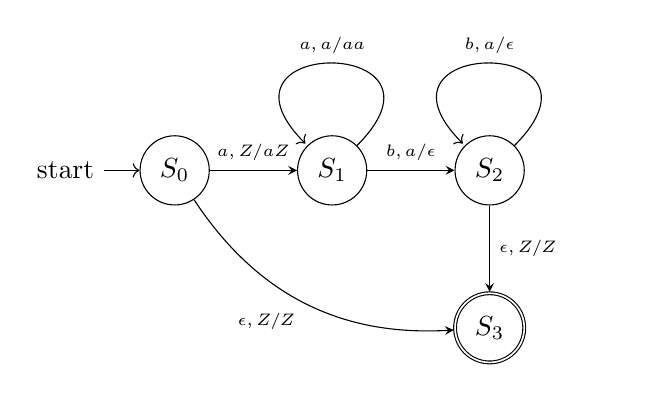
\begin{tikzpicture}
    \node (S0) [state, initial] {$S_{0}$};
    \node (S1) [state] at (2,0) {$S_{1}$};
    \node (S2) [state] at (4,0) {$S_{2}$};
    \node (S3) [state, accepting] at (4,-2) {$S_{3}$};

    \path (S0) [-stealth] edge node[above] [font=\fontsize{6}{12}\selectfont] {$a,Z/aZ$} (S1);
    \path (S0) [-stealth, bend right] edge node[below left] [font=\fontsize{6}{12}\selectfont] {$\epsilon,Z/Z$} (S3);
    \path (S1) [-stealth, loop] edge node[above] [font=\fontsize{6}{12}\selectfont] {$a,a/aa$} (S1);
    \path (S1) [-stealth] edge node[above] [font=\fontsize{6}{12}\selectfont] {$b,a/\epsilon$} (S2);
    \path (S2) [-stealth, loop] edge node[above] [font=\fontsize{6}{12}\selectfont] {$b,a/\epsilon$} (S2);
    \path (S2) [-stealth] edge node[right] [font=\fontsize{6}{12}\selectfont] {$\epsilon,Z/Z$} (S3);
\end{tikzpicture}

\end{document}
